\chapter{Kiến thức nền tảng}

Để có thể nghiên cứu bài toán nhận diện vật thể trong ảnh, những kiến thức nền tảng quan trọng nhóm cần phải nắm bao gồm:
\begin{itemize}
	\item Convolution Neural Network.
	\item Các kiến trúc mạng CNN nâng cao
\end{itemize}

\section{Khái niệm chung}

Mạng nơ-ron nhân tạo (Artificial Neural Network- ANN) hay thường gọi ngắn gọn là mạng nơ-ron là một mô hình toán học hay mô hình tính toán được xây dựng dựa trên các mạng nơ-ron sinh học, bao gồm có một nhóm các nơ-ron nhân tạo (nút: node) nối với nhau và xử lý thông tin bằng cách truyền theo các kết nối và tính giá trị mới tại các nút. Trong nhiều trường hợp, mạng nơ-ron nhân tạo là một hệ thống thích ứng (adaptive system) tự thay đổi cấu trúc của mình dựa trên các thông tin bên ngoài hay bên trong chảy qua mạng trong quá trình học.

	Trong thực tế sử dụng, nhiều mạng nơ-ron là các công cụ mô hình hóa dữ liệu thống kê phi tuyến. Chúng có thể được dùng để mô hình hóa các mối quan hệ phức tạp giữa dữ liệu vào và kết quả hoặc để tìm kiếm các dạng/mẫu trong dữ liệu. ANN giống như bộ não con người, được học bởi kinh nghiệm (thông qua huấn luyện), có khả năng lưu giữ những kinh nghiệm tri thức và sử dụng những tri thức đó trong việc dự đoán các dữ liệu chưa biết (unseen data). Kiến trúc chung của một mạng nơron nhân tạo (ANN) gồm 3 thành phần đó là: lớp đầu vào (input layer), lớp ẩn (hidden layer) và lớp đầu ra (output layer).

Khi ta áp dụng mạng ANN lên dữ liệu ảnh đầu vào có kích thước mxn. Với một hidden layer, có một nơ-ron ta sẽ có số trọng số $w_{ij}$ phải lưu là mxn trọng số. Từ đó ta có thể thấy với một ảnh có kích thước 50x50 thì với mạng như trên ta đã phải nhớ đến 2500 trọng số $w_{ij}$. Thế nhưng ảnh bình thường lại có kích thước lớn hơn 50x50 và mạng ANN với một lớp ẩn và một nơ-ron thì kết quả học sẽ không được tốt. Vậy nên khi áp dụng ANN lên dữ liệu ảnh ta sẽ phải nhớ rất nhiều trọng số $w_{ij}$, vì vậy khó có thể tạo được một mạng có độ sâu đủ lớn để áp dụng lên dữ liệu ảnh.

Convolutional  Neural  Network  (CNNs - Mạng neural tích chập) là một trong những mô hình Deep Learning tiên tiến giúp cho chúng ta xây dựng được những hệ thống thông minh với độ chính xác cao.
\section{Convolution Neural Network \cite{cnn}}

\subsection{Các thành phần cơ bản của mạng CNN}

Các thành cơ bản của CNN gồm:
\begin{itemize}
	\item Tầng Convolution
	\item Pooling
	\item ReLU
	\item Fully Connected
\end{itemize}
 
Một vài khái niệm cần hiểu:
\begin{itemize}
	\item Feature: CNNs so sánh hình ảnh theo từng mảnh. Các mảnh (thuộc tính đặc trưng) mà nó tìm được gọi là các feature. Bằng cách tìm ở mức thô các feature khớp nhau ở cùng vị trí trong hai hình ảnh, CNNs nhìn ra sự tương đồng tốt hơn nhiều so với việc khớp toàn bộ bức ảnh. Mỗi feature giống như một hình ảnh mini - một mảng hai chiều nhỏ. Các feature khớp với các khía cạnh chung của các bức ảnh.
\begin{center}
    \begin{figure}[h!p]
    \begin{center}
     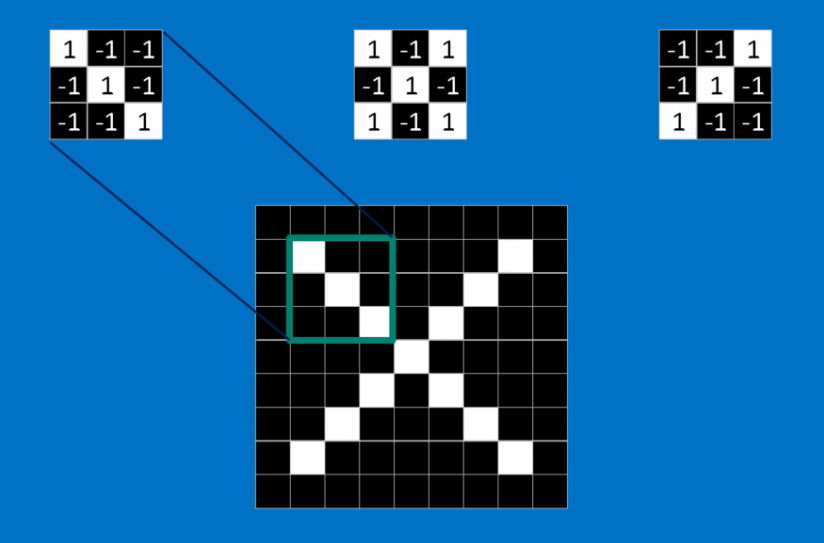
\includegraphics[scale=.5]{img/feature.png}
    \end{center}
    \caption{Đặc trưng - Feature trong CNN \cite{cnn}}
    \label{refhinh1}
    \end{figure}
\end{center}
	\item Bộ lọc (filter): là một ma trận có kích thước nhỏ thường là 3x3 hoặc 5x5, được khởi tạo ban đầu. Khi “trượt” filter trên ảnh đầu vào ứng với mỗi vùng trượt sẽ có một nơ-ron ẩn trong lớp ẩn (hidden layer) đầu tiên, quá trình này được lặp lại liên tục đến khi trượt xong toàn bộ bức ảnh cuối cùng ta sẽ được 1 feature map. Tuy nhiên trong thực tế chúng ta cần rất nhiều feature map.
	\begin{center}
    \begin{figure}[h!]
    \begin{center}
     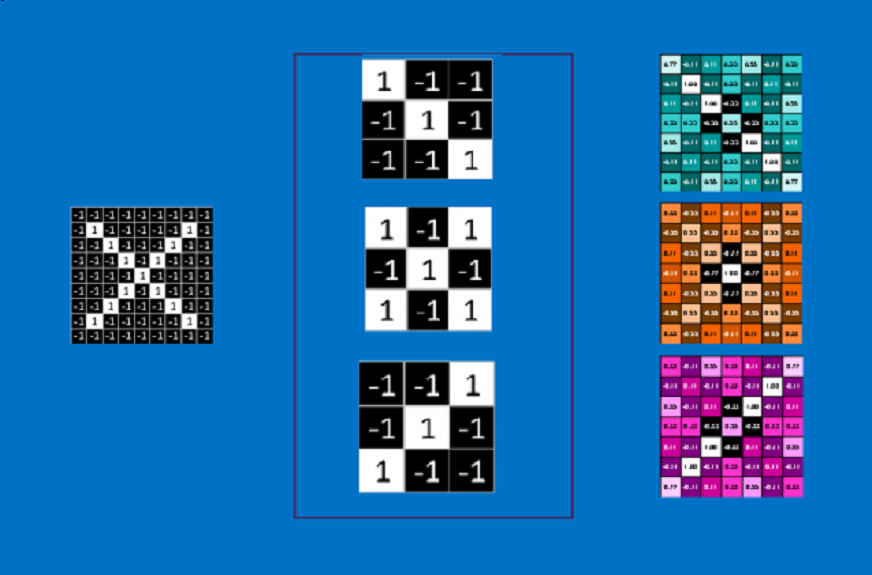
\includegraphics[scale=0.5]{img/convolution_3.png}
    \end{center}
    \caption{Bộ lọc trong CNN \cite{cnn}} 
    \label{refhinh4}
    \end{figure}
\end{center}
	\end{itemize}


\subsubsection{Tầng Convolution}

Lớp convolution sử dụng bộ lọc (filters) có kích thước nhỏ hơn so với ảnh (thường ma trận 3x3 hoặc 5x5), tiến hành tích chập. Bộ filter sẽ dịch chuyển trên ảnh theo bước trược chạy dọc theo ảnh và quét toàn bộ ảnh thu được feature map.

\begin{center}
    \begin{figure}[h!]
    \begin{center}
     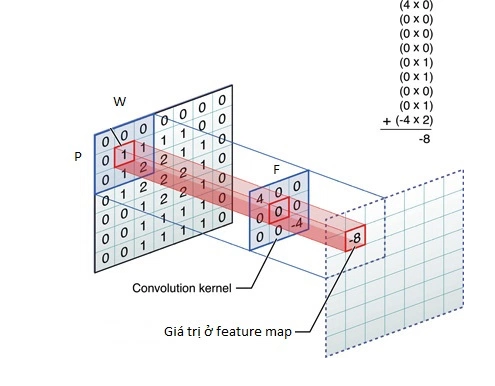
\includegraphics[scale=0.7]{img/convolution_1.png}
    \end{center}
    \caption{Tầng Convolution trong CNN \cite{tangconv}}
    \label{refhinh2}
    \end{figure}
\end{center}

Tính toán sự khớp của một feature đối với một hình ảnh, ta thực hiện nhân mỗi điểm ảnh trong feature với giá trị của điểm ảnh tương ứng trong hình ảnh. Cộng tổng lại và chia cho số lượng điểm ảnh trong feature.
\begin{center}
    \begin{figure}[h!]
    \begin{center}
     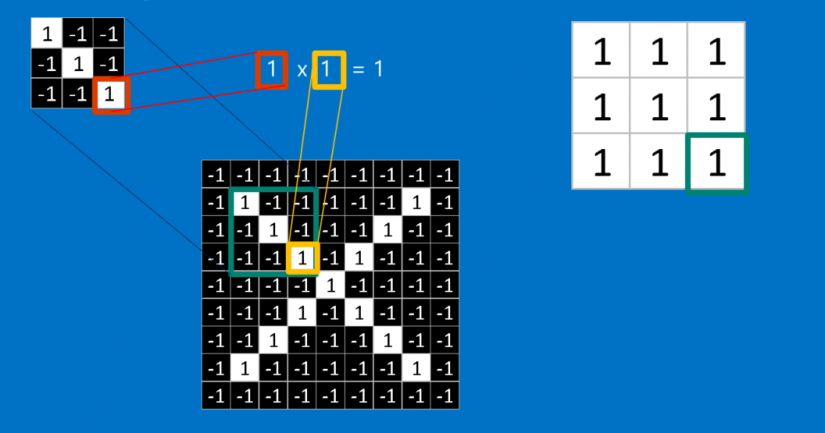
\includegraphics[scale=0.5]{img/convolution_2.png}
    \end{center}
    \caption{Ví dụ mẫu tính toán tích chập \cite{cnn}}
    \label{refhinh3}
    \end{figure}
\end{center}

Ví dụ trong hình mẫu: nếu giá trị điểm ảnh trong feature khớp màu với điểm ảnh trong hình sẽ cho giá trị là 1 (1x1=1 hoặc (-1)x(-1) = 1), nếu giá trị điểm ảnh không khớp màu sẽ cho giá trị (-1) (1 x (-1) =(-1)). Cộng các kết quả lại, chia cho số lương điểm ảnh của feature 3x3=9.

Một mạng tích chập cần nhiều feature map, thực hiện tương tự quá trình tích chập cho từng feature khác, kết quả thu được là một tập hợp các hình ảnh được lọc, tương ứng với mỗi filter.
Chú ý: các giá trị gần 1 cho thấy sự khớp mạnh, các giá trị gần -1 cho thấy sự khớp mạnh với âm bản của feature, và các giá trị gần bằng 0 cho thấy không khớp với bất kỳ loại nào.

Thực hiện tương tự quá trình tích chập cho từng feature khác, kết quả thu được là một tập hợp các hình ảnh được lọc, tương ứng với mỗi filter.

Có hai dạng tính Convolution chính mà ta thường dùng là Valid và Same. Hai dạng cho ảnh kết quả có kích thước khác nhau:
\begin{itemize}
\item Dạng Valid: kernel được trượt trên toàn ảnh, sau khi tính tích chập (convolution) kết quả sẽ nhỏ hơn kích thước ảnh ban đầu. Với ảnh đầu vào có kích thước m x m, kernel kích thước nxn thì ảnh đầu ra sẽ có kích thước (m n + 1)x(m n + 1).
\item Dạng Same: trước khi tính Convolution,  ảnh sẽ được đệm (padding) thêm các giá trị (thường các giá trị này sẽ là 0 hoặc 1) để tăng kích thước ảnh, sao cho sau khi thực hiện Convolution, kích thước ảnh kết quả sẽ bằng với kích thước ảnh ban đầu.

Về mặt toán học, cho hàm f(x), tích chập của f với hàm k(x) được tính như sau:
\begin{equation}
r(x) = (f*k)(x) =\int f(x - n)k(n) dn
\end{equation}
\end{itemize}

Thực hiện "trượt" hàm k(x) lên hàm f(x) và tính tổng phần chồng lấp của 2 hàm này với nhau, do đó kết quả của phép tích chập là ta được một hàm mới là sự "hoà trộn" của k(x) vào f(x). Trong trường hợp rời rạc, phép tích phân trở thành tổng:
\begin{equation}
r(i) = (f*k)(i) =\sum f(i - n)k(n)
\end{equation}
Với trường hợp 2 chiều, ta chỉ cần thêm chỉ số cho chiều thứ 2:
\begin{equation}
r(i, j) = (f*k)(i, j) =\sum\sum f(i - n, j- m)k(n, m)
\end{equation}
\subsubsection{Lớp gộp Pooling}

Pooling layer trong mạng CNN giúp loại bỏ những thông tin không cần thiết, rất hữu ích khi ảnh có kích cỡ lớn (dimentional reduction) làm giảm độ phức tạp khi tính toán. Tuy nhiên nếu lạm dụng nhiều có thể làm mất dữ liệu. Trong lóp này sử dụng cửa sổ trượt (thường là 2x2), mỗi lần trượt theo một bước trượt (stride) cho trước . Khác với lớp Convolutional, lớp Pooling không tính tích chập mà tiến hành lấy mẫu (subsampling). Một giá trị đại diện thông tin ảnh tại vùng ảnh đó được giữ lại. Một số phương pháp phổ biến được sử dụng trong lớp Pooling là MaxPooling (lấy giá trị lớn nhất), MinPooling (lấy giá trị nhỏ nhất) và AveragePooling (lấy giá trị trung bình).
\begin{center}
    \begin{figure}[h!]
    \begin{center}
     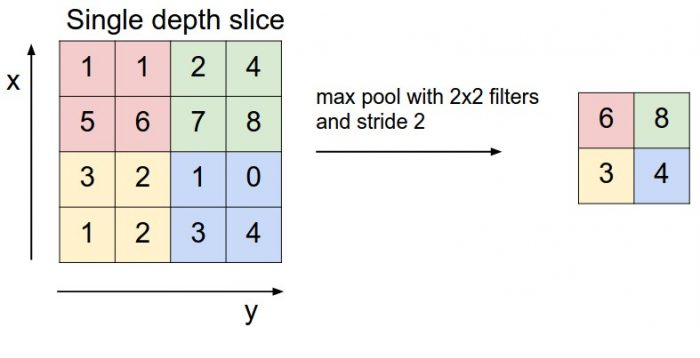
\includegraphics[scale=0.5]{img/MaxPooling.png}
    \end{center}
    \caption{Max Pooling trong CNN \cite{maxpool}}
    \label{refhinh5}
    \end{figure}
\end{center}

Ví dụ minh họa: mô hình có kích thước 32x32 (hình minh họa trên), lớp Pooling dùng filter kích thước 2x2, bước trượt (stride) là 2, sử dụng phương pháp MaxPooling. Tiến hành gộp ảnh, giá trị lớn nhất trong vùng cửa sổ 2x2 giới hạn bởi filter được giữ lại, làm đầu ra. Sau lớp Pooling, kích thước ảnh giảm đi 2 lần mỗi chiều (16x16).

Khi dữ liệu ảnh có kích thước lớn, thực hiện qua nhiều lớp Pooling sẽ thu nhỏ, giảm kích thước dữ liệu làm giảm lượng tham số, tăng hiệu quả tính toán và góp phần kiểm soát hiện tượng quá khớp (overfitting).
\newpage
\subsubsection{Rectified Linear Units - ReLU}

Hay còn gọi là hàm tinh chỉnh các đơn vị tuyến tính

Đóng vai trò nhỏ nhưng quan trọng trong quá trình là Rectified Linear Unit hoặc ReLU. Lớp này thường được cài đặt sau lớp Convolutional. Có nhiệm vụ chuyển toàn bộ giá trị âm của kết quả từ lớp Convolutional thành giá trị 0, sử dụng hàm kích hoạt $ f(x) = max(0,x)$. RELU giúp tạo nên tính phi tuyến cho mô hình, giữ vững sự tin cậy toán học giúp các giá trị khỏi bị mắc kẹt gần 0 hoặc bị về vô tận.

Ngoài ra còn một số hàm truyền khác:
\begin{center}
    \begin{figure}[h!]
    \begin{center}
     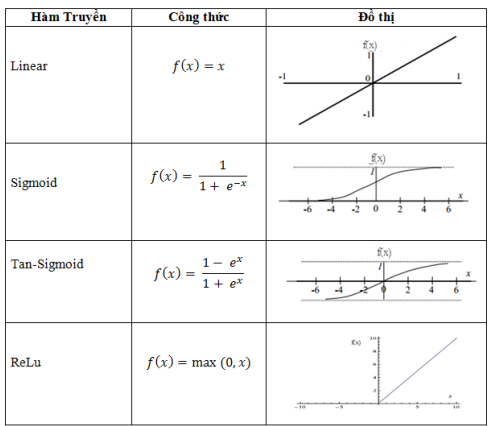
\includegraphics[scale=1]{img/RELU.png}
    \end{center}
    \caption{Các hàm truyền trong CNN \cite{softmax} }
    \label{refhinh6}
    \end{figure}
\end{center}
\newpage
\subsubsection{Fully-connected Layer}

\begin{center}
    \begin{figure}[h!]
    \begin{center}
     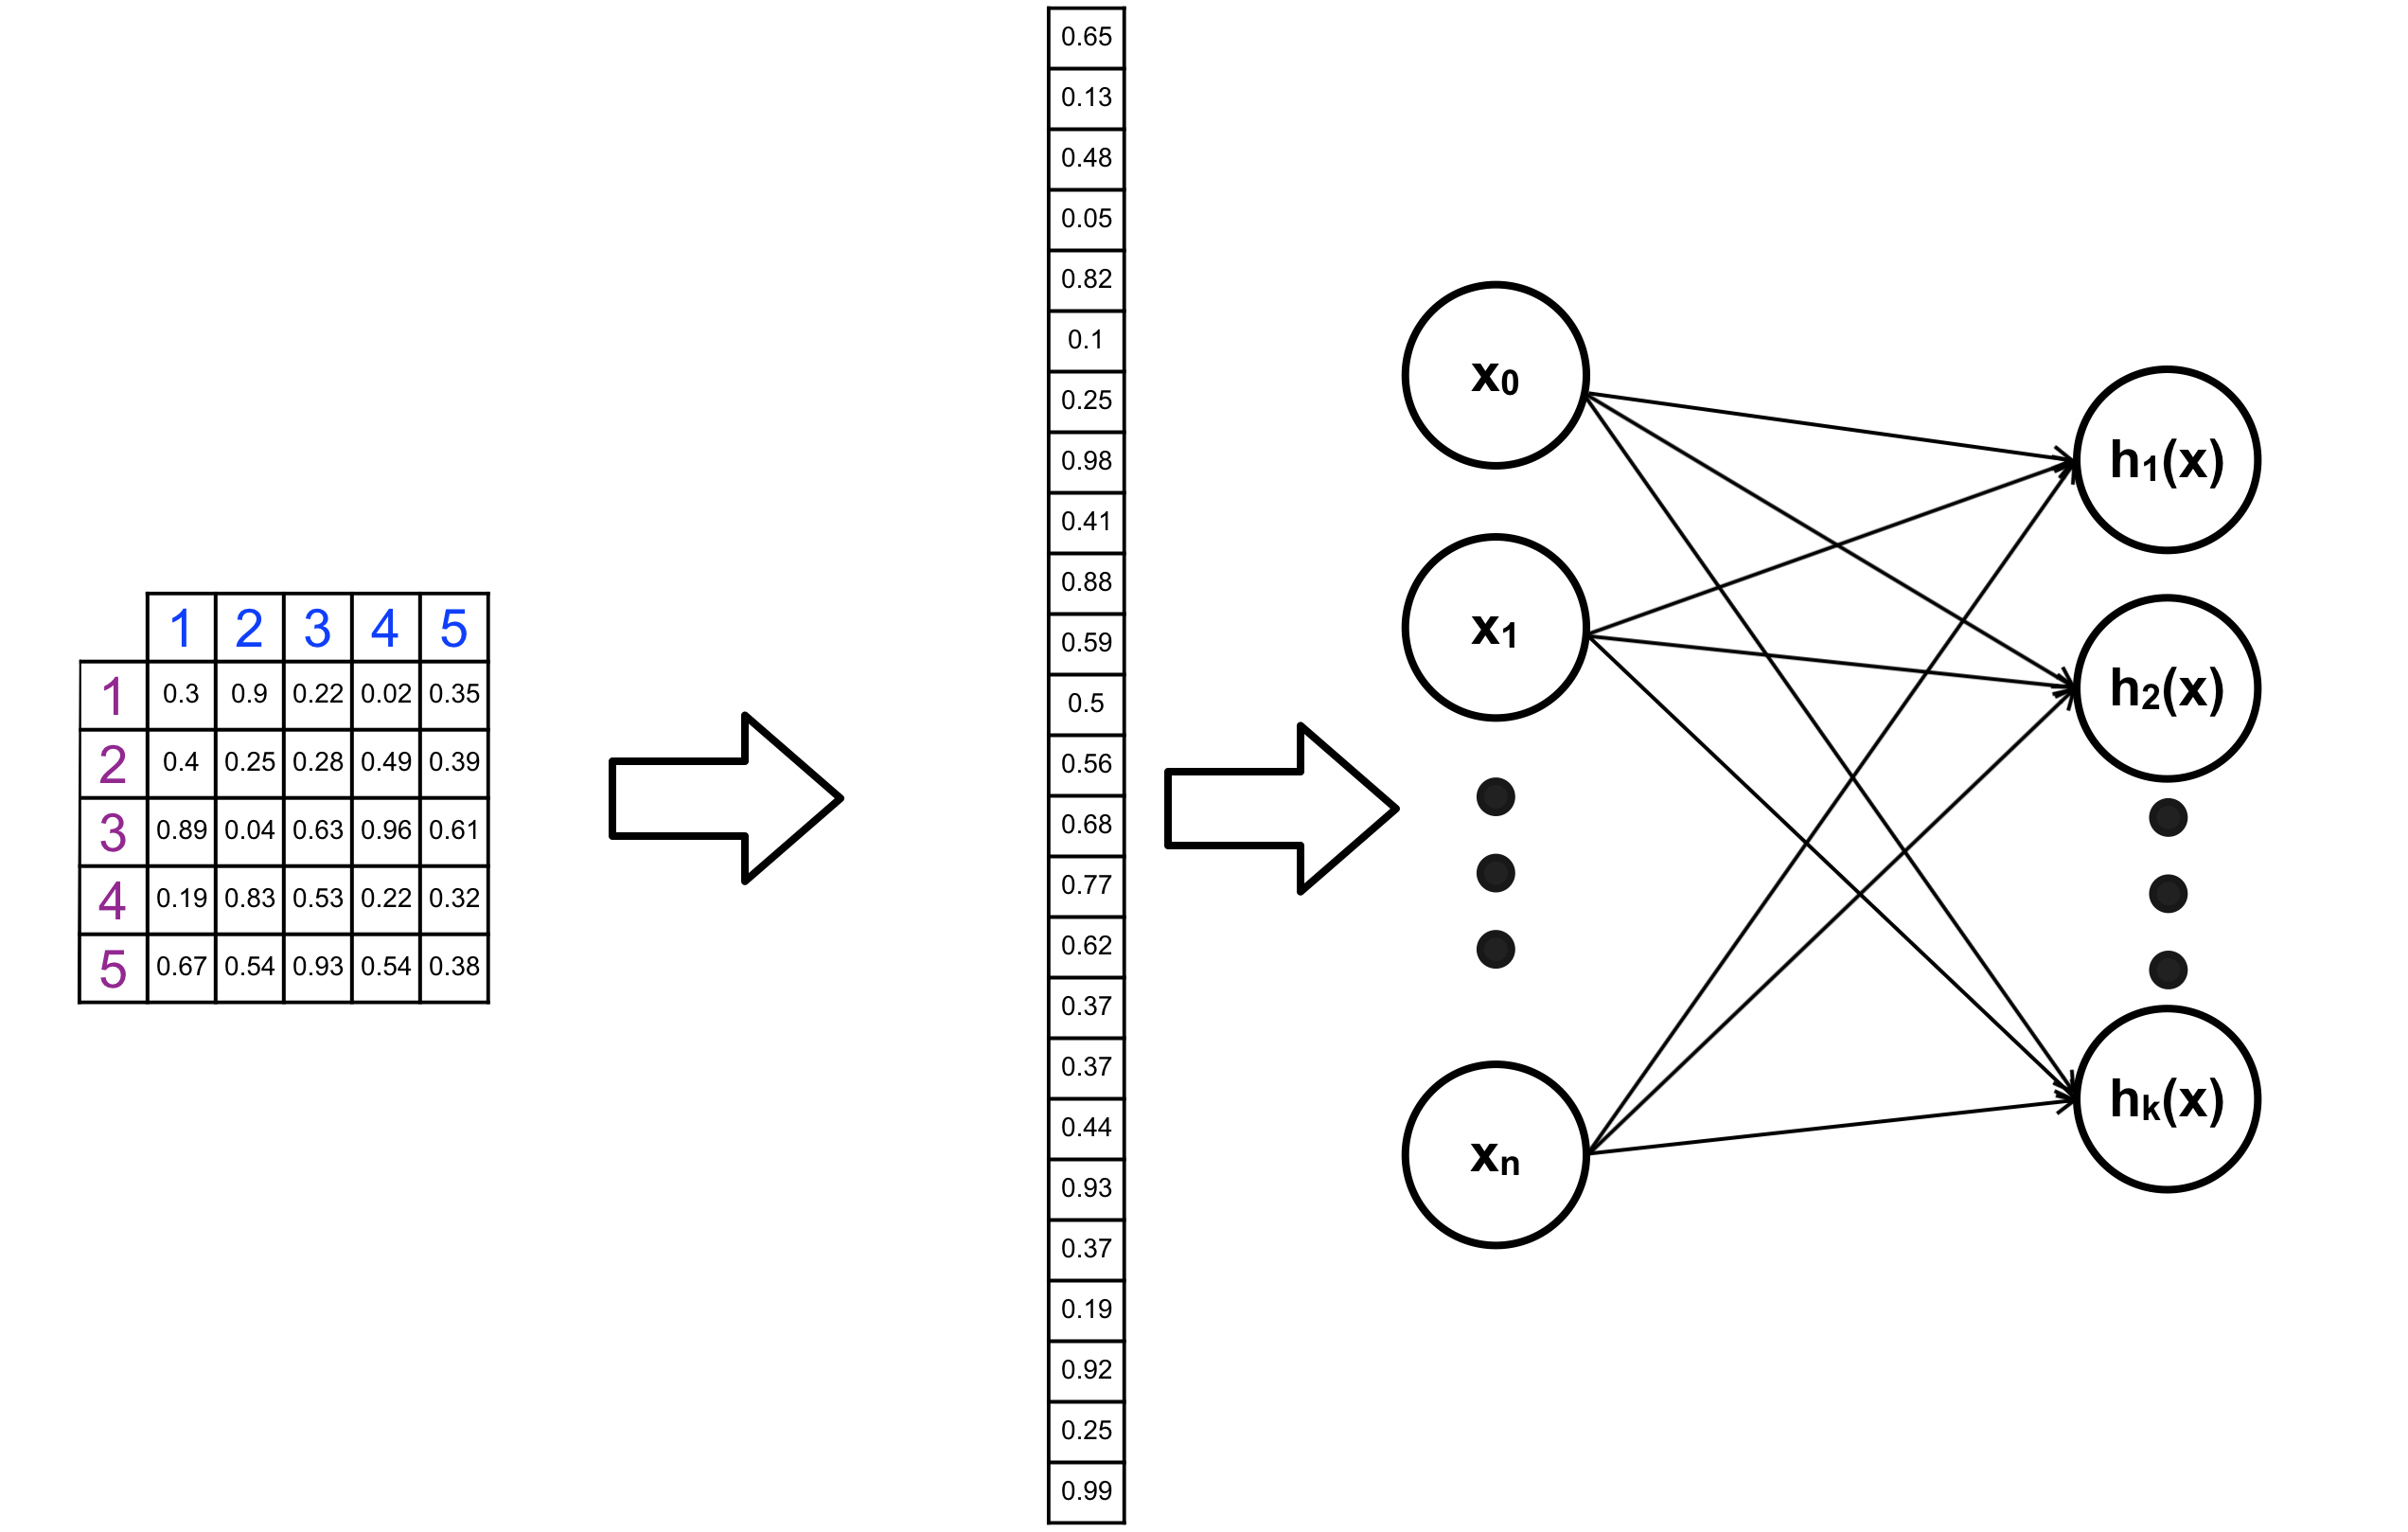
\includegraphics[scale=0.25]{img/Fully-Connected_Layer.png}
    \end{center}
    \caption{Tầng kết nối đầy đủ \cite{fullconnect} }
    \label{refhinh7}
    \end{figure}
\end{center}

Fully-Connected Layer (FC Layer) chính là một mạng NN được gắn vào phần cuối của CNNs. Lớp này tương tự với lớp trong mạng nơ-ron truyền thẳng, các giá trị điểm ảnh liên kết với nhau liên tiếp. Sau khi được xử lý, rút trích, gộp,... từ các lớp trước đó, dữ liệu ảnh không còn quá lớn nên có thể áp dụng mô hình truyền thẳng. Các layer được kết nối đầy đủ lấy các hình ảnh đã lọc ở cấp cao và chuyển thành các phiếu bầu (vote). Thay vì coi đầu vào như một mảng hai chiều, chúng được coi như mảng một chiều và tất cả đều được xử lý giống nhau. Mỗi giá trị hướng đến kết quả cho hình ảnh hiện tại. Tuy nhiên, trong quá trình này các giá trị có mức độ quyết định không giống nhau. Một số giá trị cho biết kết quả của hình ảnh này là tốt hơn nhiều so với những giá trị khác, và một số lại đặc biệt tốt khi cho biết kết quả khác, thể hiện qua trọng số (weight), hoặc là mức độ kết nối...

Như vậy, lớp fully-connected có vai trò như một mô hình phân lớp và thực hiện phân lớp dữ liệu đã được xử lý thông qua các lớp trước đó.

\subsection{Kiến trúc mạng CNN cơ bản}

\begin{center}
    \begin{figure}[h!]
    \begin{center}
     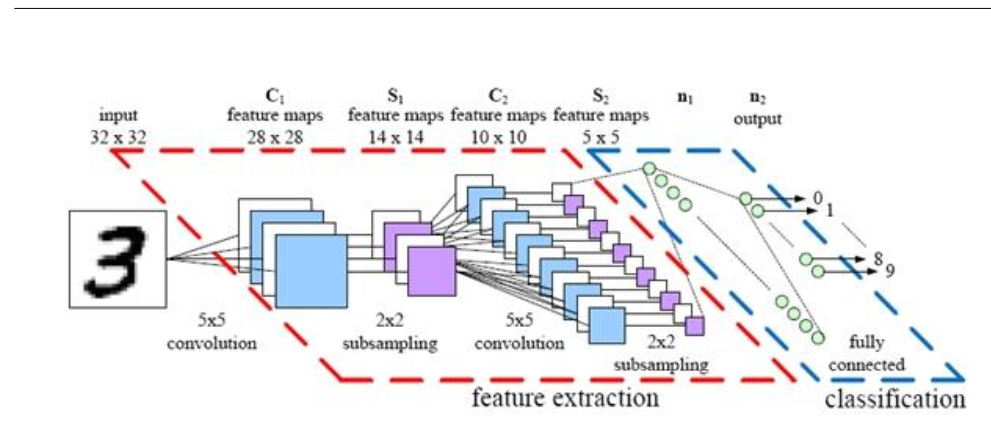
\includegraphics[scale=0.5]{img/basiccnn1.png}
    \end{center}
    \caption{Kiến trúc mạng CNN cơ bản \cite{mangcnn} } 
    \label{refhinh8}
    \end{figure}
\end{center}

Trong mô hình CNN hai khía cạnh cần quan tâm là tính bất biến (Location Invariance) và tính kết hợp (Compositionality). Cùng một đối tượng mẫu, nếu đối tương được chiếu theo các hướng khác nhau (dịch (translation), quay (rotation), co giãn (scaling)) cũng ảnh hưởng đến kết quả thuật toán, độ chính xác sẽ bị ảnh hưởng. Pooling layer tạo nên tính bất biến với các phép biến đổi của ảnh, vật: phép dịch (translation), phép quay (rotation) và phép co giãn (scaling). Tính kết hợp thể hiện qua việc thông qua việc càng nhiều thông tin bổ sung kết quả dữ liệu cho ta đầu ra càng chính xác, như mạng nơ-ron tích chập được hình thành từ việc ghép bổ xung nhiều feature map.

Mô hình bắt đầu với lớp Convolutional. Lớp RELU thường luôn được cài đặc ngay sau lớp Convolutional hoặc kết hợp cả hai lớp này thành một lớp. Các lớp tiếp theo có thể là Convolutional hay Pooling tùy theo kiến trúc muốn xây dựng. Cuối cùng sẽ là lớp fully-connected để tiến hành phân lớp, đưa ra kết quả đầu ra của mô hình.

Xét một kiến trúc sau đây:

Conv1 (with RELU) – Pooling – Conv2 (with RELU) – Pooling – FC – FC

Hình ảnh cần nhận dạng có kích thước 32x32. Ảnh sẽ được đưa vào lớp Conv1 (Convolutional kết hợp RELU) gồm 32 filter có kích thước 5x5, thực hiện tính tích chập với 32 filter ta sẽ có 32 ảnh kết quả.

\begin{center}
    \begin{figure}[h!]
    \begin{center}
     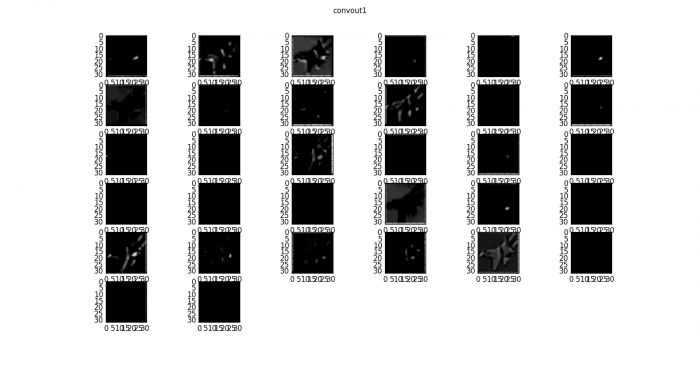
\includegraphics[scale=0.8]{img/basiccnn2.png}
    \end{center}
    \caption{Nhận diện hình ảnh với CNN \cite{ptha} }
    \label{refhinh9}
    \end{figure}
\end{center}

Mỗi ảnh sẽ có kích thước tương ứng là 28x28. Sau đó cho qua lớp Pooling và kết quả trả ra sẽ là 32 ảnh có kích thước 14x14. Tiếp tục cho dữ liệu đi vào lớp Conv2. Tương tự như Conv1, ảnh sẽ được tính tích chập với filter và trả ra kết quả. Lớp Pooling tiếp theo sẽ tiếp tục giảm kích thước của ảnh xuống còn 5x5. Với kích thước đủ nhỏ, lớp Fully-connected tiếp theo sẽ xử lý và đưa ra kết quả phân lớp hay kết quả nhận dạng.

\subsubsection{Lan truyền ngược (Backpropagation)}

Câu hỏi đặt ra: Các feature đến từ đâu? Làm thế nào để tìm trọng số trong các layer được kết nối đầy đủ?

Thuật toán Back – Propagation được sử dụng để điều chỉnh các trọng số kết nối sao cho tổng sai số e nhỏ nhất.

\begin{equation}
E = \sum_{i = 1}^n (t(x_i, w) - y(x_i))^2
\end{equation}

Trong đó:

\qquad $t(x_i, w)$: giá trị của tập mẫu

\qquad $(y(x_i))$: giá trị kết xuất của mạng

Mỗi nơron đều có giá trị vào và ra, mỗi giá trị đều có một trọng số để đánh giá mức độ ảnh hưởng của giá trị vào đó. Thuật toán Back –Propagation sẽ điều chỉnh các trọng số đó để giá trị $ e_j = t_j - y_j $ là nhỏ nhất.

Xác định vị trí của mỗi nơron, nơron nào là của lớp n và nơron nào là của lớp xuất.

Các ký hiệu:

\qquad $W_{ij} $: vector trọng số của nơron j số đầu vào i

\qquad $u_j$ : vector giá trị kết xuất của nơron trong lớp j

Giá trị sai số của nơron j tại vòng lặp thứ n\\
\begin{equation}
e_j(n) = t_j(n) - y_j(n)
\end{equation}
Tổng bình phương sai số của mạng nơron:\\
\begin{equation}
E(n) = \frac{1}{2}\sum_{j= 1}^k e_j^2 (n)
\end{equation}
Tổng trọng số input tại nơron j:\\
\begin{equation}
u_j(n) = \sum_{i = 0}^pw_{ij}x_j(n)
\end{equation}
Giá trị kết xuất của neeural j:\\
\begin{equation}
y_j(n) = f_j(u_j(n))
\end{equation}
Tính toán giá trị đạo hàm sai số cho mỗi neural $w_{ij}$:
\begin{equation}
\frac{\partial E(n)}{\partial W_{ij}(n)} = \frac{\partial E(n)}{\partial e_j(n)}\frac{\partial e_j(n)}{\partial y_j(n)}\frac{\partial y_j(n)}{\partial u_j(n)}\frac{\partial u_j(n)}{\partial w_j(n)}
\end{equation}
Trong đó 
\begin{equation} 
\frac{\partial E(n)}{\partial e_j(n)}=\frac{\frac{1}{2} \sum_{j=1}^k e_j^2(n) }{\partial e_j(n)} = \partial e_j(n)
\end{equation}
\begin{equation} 
\frac{\partial e_j(n)}{\partial y_j(n)}=\frac{\partial(t_i(n) - y_i(n))}{\partial y_j(n)} = -1;
\end{equation}
\begin{equation} 
\frac{\partial y_j(n)}{\partial u_j(n)}=f'_j(u_j(n))
\end{equation}
\begin{equation} 
\frac{\partial u_j(n)}{\partial w_j(n)}=\frac{\partial (\sum_{i = 0}^p W_{ij} x_i(n))}{\partial w_{ij}(n)}= x_i(n)
\end{equation}
\begin{equation} 
=>\frac{\partial E(n)}{\partial w_{ij}(n)} = -e_j(n).f'(u_j(n))x_i(n)
\end{equation}

Giá trị điều chỉnh trọng số:

Để cập nhật trọng số $w_{ij}$: chọn một tốc độ học: $\eta$. Tính tích của tốc độ học với gradient, nhân (-1).
\begin{equation}
\Delta w_{ij} = -\eta \frac{\partial E(n)}{\partial w_{ij}(n)}=-\eta e_j(n).f'(u_j(n))x_i(n)\\
\end{equation}

Trong đó
\begin{equation}
\partial _j = \frac{\partial E(n)}{\partial W_{ij}(n)} =  \frac{\partial E(n)}{\partial e_j(n)}\frac{\partial e_j(n)}{\partial y_j(n)}\frac{\partial y_j(n)}{\partial u_j(n)}=e_j(n).f'(u_j(n))
\end{equation}
\begin{equation}
\Delta w_{ij} = -\eta \delta _j(n)x_i(n)
\end{equation}

Công thức điều chỉnh trọng số:

\begin{equation}
w_{ij(n+1)} =w_{ij}(n)+ \Delta w_{ij}(n) 
\end{equation}

\section{Các kiến trúc mạng CNN nâng cao}
\subsection{Mạng LeNet-5}

Năm 1994 tác phẩm tiên phong của Yann LeCun được đặt tên là LeNet5 sau nhiều lần lặp lại thành công trước đó kể từ năm 1988. Và đây là một trong những mạng thần kinh xoắn nếp đầu tiên, giúp đẩy mạnh lĩnh vực học tập sâu.

Vào thời điểm đó không có GPU để huấn luyện, và thậm chí cả CPU cũng chậm. Vì vậy, có thể lưu các thông số và tính toán là một lợi thế quan trọng. Kiến trúc LeNet là  đơn giản và  nhỏ gọn (về bộ nhớ), làm cho nó  hoàn hảo để giảng dạy những điều cơ bản của CNN - nó thậm chí có thể chạy trên CPU (nếu hệ thống của bạn không có GPU thích hợp).

\begin{center}
    \begin{figure}[h!]
    \begin{center}
     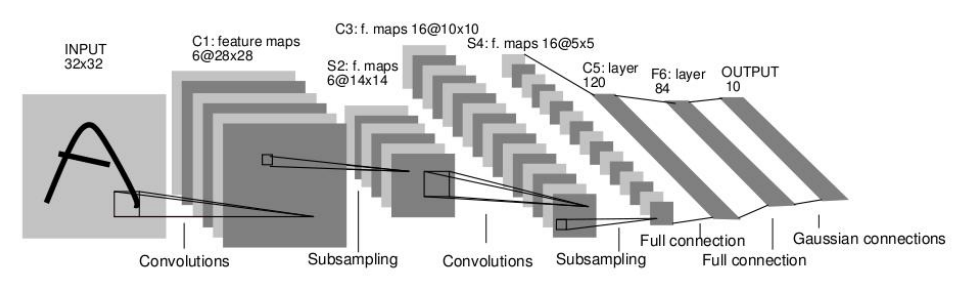
\includegraphics[scale=0.5]{img/lenet.png}
    \end{center}
    \caption{Mô hình mạng LeNet \cite{lenet5}}
    \label{refhinh10}
    \end{figure}
\end{center}

Các đặc điểm của LeNet5 có thể được tóm tắt như sau \cite{lenet5}:

\begin{itemize}
\item Chuỗi sử dụng mạng nơ-ron thần kinh gồm 3 lớp: xoắn chập (convolution), tập hợp gộp (pooling), phi  tuyến (non-linearity).
\item Sử dụng chập (convolution) để chiết xuất các đặc tính không gian.
\item Phi tuyến dùng tanh hoặc sigmoids
\item Mạng nơ-ron đa lớp (multi-layer neural network MLP) làm phân loại cuối cùng (final classifier).
\item Ma trận kết nối thưa thớt giữa các lớp để tránh chi phí tính toán lớn.
\item Hàm gộp lấy giá trị trung bình (Average pooling).
\end{itemize}

Thực hiện:

Đầu vào là một ảnh 32x32, thực hiện tích chập (convolution) dùng bộ lọc (filter) là 5x5, với 6 feature để có được một khối lớp (layer) kết quả là 28x28x6. Sau đó, chúng ta tiến hành lấy mẫu (subsampling) để có được lượng kích hoạt 14x14x6: giảm một nửa chiều rộng của ảnh, sử dụng  ma trận 2x2.  Tiếp tục tích chập với 16 ma trận tính năng để có được kích hoạt 10x10x16, dùng các bộ lọc kích thước 5x5. Thực hiện một lần nữa tiến trình lấy mẫu (subsampling), kích thước tổng hợp là 2x2. Lớp xoắn cuối cùng là 120 bộ lọc (filter) có kích thước 5x5, và làm phẳng khối lượng kích hoạt thành một vector. Cuối cùng, chúng ta thêm một lớp ẩn với 84 nơ-ron và lớp đầu ra với 10 nơ-ron.

\subsection{Mạng AlexNet}

Sơ  lược về AlexNet đây là mô hình đánh dấu sự phổ biến của CNN, dành chiến thắng trong cuộc thi ILSVRC 2012 (ImageNet Large Scale Visual Recognition Challenge - một cuộc thi thế vận hội cho thị giác máy tính nơi mà các đội trên thế giới cạnh tranh nhau về mô hình thị giác máy tính theo các nhiệm vụ như phân loại, phát hiện, ...)

Điều đáng nói ở mạng này là chỉ nhận dữ liệu đầu vào là dữ liệu thô và không áp dụng phương pháp trích đặc trưng nào.

\begin{center}
    \begin{figure}[h!]
    \begin{center}
     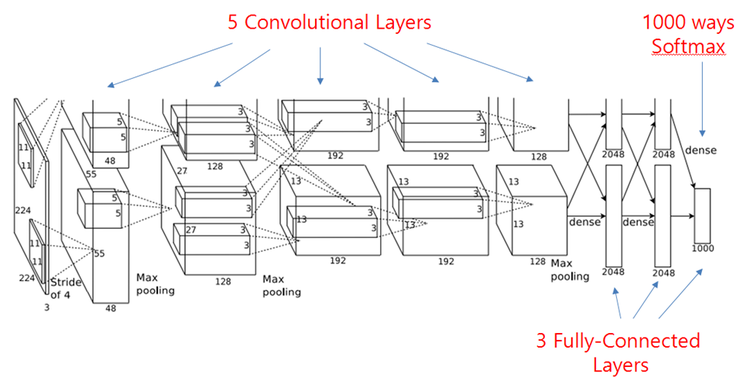
\includegraphics[scale=0.5]{img/alexnet2.png}
    \end{center}
    \caption{Mạng AlexNet \cite{lenet5}}
    \label{refhinh13}
    \end{figure}
\end{center}

Một số thông số cơ bản trong một mạng Alexnet \cite{alexnet}

\begin{itemize}
\item Tầng 0: Hình ảnh đầu vào
\begin{itemize}
\item Size: 227 x 227 x 3
\end{itemize}
\item Tầng 1: Mạng tích chập với 96 bộ lọc, kích thước 11x11, bước trượt (stride) S = 4, bộ đệm P = 0
\begin{itemize}
\item Kích thước: 55 x 55 x 96
\item (227 - 11)/4 + 1 = 55 size của đầu ra
\item Độ sâu 96 bởi vì 1 tập biểu thị một bộ lọc và có 96 bộ lọc
\end{itemize}
\item Tầng 2: Hàm tổng hợp tối đa (max-pooling) với bộ lọc có kích thước 3x3, bước trượt S = 2
\begin{itemize}
\item Kích thước: 27 x 27 x 96
\item (55 - 3)/2+1 = 27 là kích thước của đầu r
\item Độ sâu 96
\end{itemize}
\item Tầng 3: Mạng tích chập với 256 bộ lọc, kích thước 5x5, bước trượt S = 1, bộ đệm P = 2
\begin{itemize}
\item Kích thước: 27 x 27 x 256
\item Padding = 2 nên kích thước ban đầu được thay đổi l
\item Độ sâu 256 vì có 256 bộ lọc
\end{itemize}
\item Tầng 4: Mạng tích chập với bộ lọc 3x3, bước trượt S = 2
\begin{itemize}
\item Kích thước: 13 x 13 x 256
\item Kích thước đầu ra: (27 - 3)/2 + 1 = 13
\item Độ sâu 256
\end{itemize}
\item Tầng 5: Mạng tích chập với 384 bộ lọc, kích thước 3x3, bước trượt S = 1, bệ đệm P = 1
\begin{itemize}
\item Kích thước: 13 x 13 x 384
\item Vì bộ đệm P = 1 nên kích thước được thay đổi
\item Độ sâu 384 vì có 384 bộ lọc
\end{itemize}
\item Tầng 6: Mạng tích chập với 384 bộ lọc, kích thước 3x3, bước trượt S = 1, bệ đệm P = 1
\begin{itemize}
\item Kích thước: 13 x 13 x 384
\item Vì bộ đệm P = 1 nên kích thước được thay đổi
\item Độ sâu 384 vì có 384 bộ lọc
\end{itemize}
\item Tầng 7: Mạng tích chập với 256 bộ lọc, kích thước 3x3, bước trượt S = 1, bệ đệm P = 1
\begin{itemize}
\item Kích thước: 13 x 13 x 384
\item Vì bộ đệm P = 1 nên kích thước được thay đổi
\item Độ sâu 256 vì có 256 bộ lọc
\end{itemize}
\item Tầng 8: Hàm tổng tối đa kích thước 3x3, bước trượt S = 2
\begin{itemize}
\item Kích thước: 6 x 6 x 256
\item Kích thước đầu ra: 6
\item Độ sâu 256
\end{itemize}
\item Tầng 9: Mạng tích chập đầy đủ với 4096 neuron
\begin{itemize}
\item Mỗi ảnh 6x6x256 = 9216 pixels được đưa vào mỗi neuron và trọng số được xác định bằng mạng truyền ngược (back - propagation)
\end{itemize}
\item Tầng 10: Mạng tích chập đầy đủ với 4096 neuron
\begin{itemize}
\item Giống tầng 9
\end{itemize}
\item Tầng 11: Mạng tích chập đầy đủ với 1000 neuron
\begin{itemize}
\item Đây là tầng cuối cùng và có 1000 neurons vì dữ liệu IAMGENET có 1000 lớp cần được phân loại
\end{itemize}
\end{itemize}

Là mạng đầu tiên làm việc tốt với tập dữ liệu IAMGENET.
\subsection{Mạng GoogLeNet}

Tổng quan về GooLeNet \cite{gglenet}
\begin{itemize}
\item Gồm 22 tầng
\item Ảnh hưởng bởi Inception module
\item Không có tầng kết nối đầy đủ (fully - connected layer)
\item Chỉ có 5 triệu thông số ít hơn so với AlexNet 12 lần
\end{itemize}


Đối với các mạng tích chập khác việc lựa chọn 3x3 hoặc 5x5 để được tối ưu là một vấn đề nan giải. Vậy thì sao chúng ta không thể sử dụng tất cả chúng, câu trả lời được hiện thực trong module Inception, ta thực hiện việc này bằng cách thực hiện từng tích chập song song và nối các kết quả lại trước khi tới lớp tiếp theo.

Đến lớp tiếp theo cũng là một module Inception, sau đó mỗi bản đồ đặc trưng (feature maps) sẽ được truyền qua hỗn hợp các xáo trộn của lớp  hiện tại. Ý tưởng là không cần phải biết trước thời gian nếu nó được tốt hơn để làm, ví dụ 3x3 sau đó là 5x5. Thay vào đó, chỉ cần làm tất cả các tích chập và để mô hình tự chọn được cái tốt nhất. Ngoài ra kiến trúc này cho phép mô hình phục hồi cả tính năng địa phương thông qua các vòng quay nhỏ hơn và các tính năng trừu tượng cao.

Inception module: thiết kế một mạng địa phương với topology và rồi đặt chúng chồng lên nhau. Tất cả các mạng tích chập được bao trong modul Inception, sử dụng hàm tinh chỉnh  đơn vị tuyến tính để kích hoạt (hàm ReLU). Tham khảo hình dưới.

Mạng gồm 22 tầng khi chỉ đếm với những tầng có thông số (nếu đếm tất cả ta có 27 tầng). Tổng số lớp (khối xây dựng độc lập) được sử dụng để xây dựng là khoảng 100 lớp. Số chính xác dựa vào cách các lớp được đếm bởi cơ sở hạ tầng học máy. Việc sử dụng tổng hợp trước khi phân loại, mặc dù việc có thêm một lớp tuyến tính. Lớp tuyến tính cho phép chúng ta dễ dàng điều chỉnh mạng với các bộ nhãn khác nhau, tuy nhiên nó được sử dụng chủ yếu để thuận tiện và mong đợi nó có một hiệu ứng lớn. Sự di chuyển từ các lớp kết nối hoàn chỉnh tới tổng hợp đã nâng cao độ chính xác lên khoảng 1\%, tuy nhiên việc sử dụng dropout vẫn là điều thiết yếu ngay cả sau khi loại bỏ các lớp kết nối hoàn toàn. 

\begin{center}
    \begin{figure}[h!]
    \begin{center}
     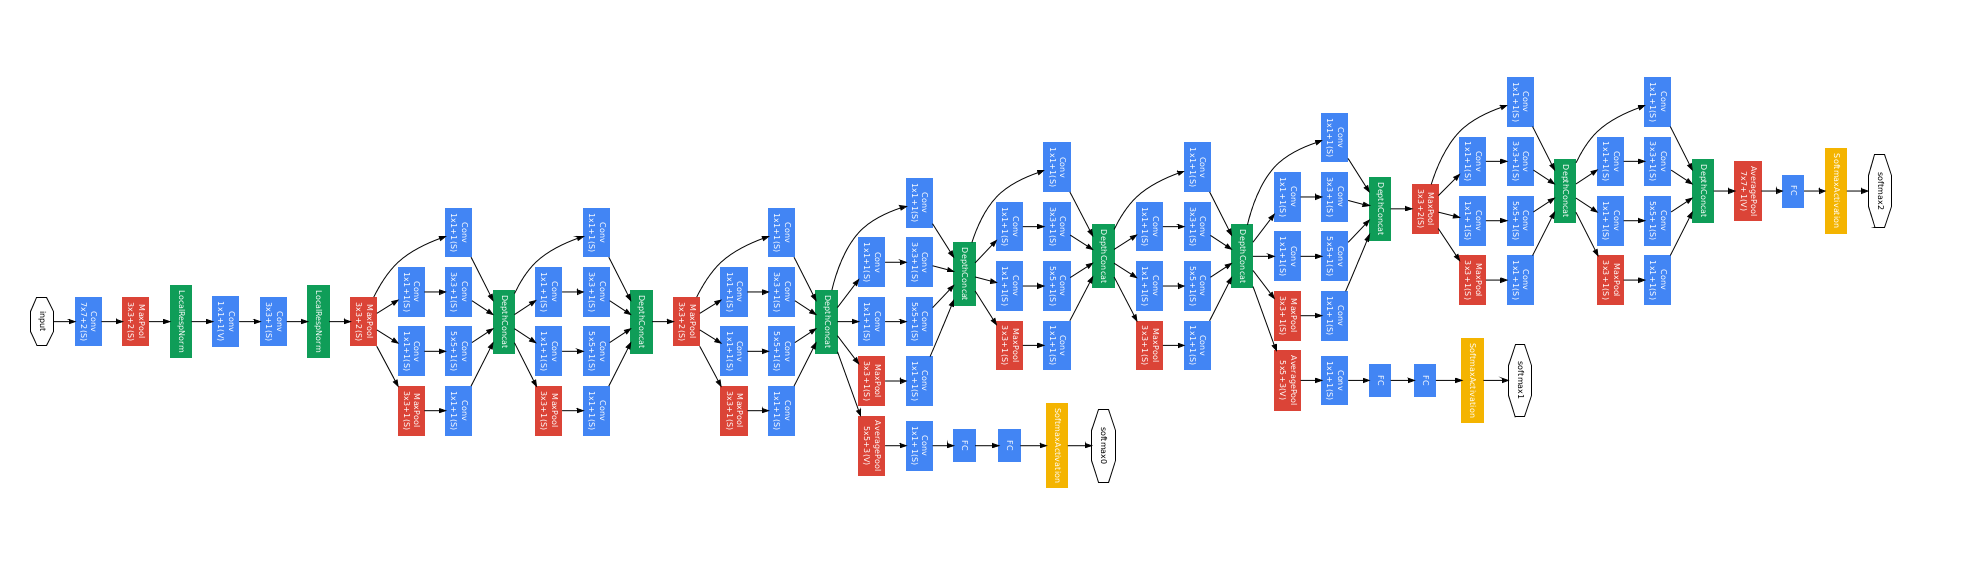
\includegraphics[scale=0.5]{img/googlenet_diagram.png}
    \end{center}
    \caption{Mô hình mạng GoogLeNet \cite{gglenet}}
    \label{refhinh12}
    \end{figure}
\end{center}

Với độ sâu  tương đối lớn của mạng, khả năng truyền của gradient trở lại tất cả các lớp một cách hiệu quả là mối quan tâm. Hiệu năng mạnh mẽ của các mạng lưới nông trên công việc này cho thấy các tính năng được sản xuất bởi các lớp ở giữa mạng nên rất phân biêt. Bằng cách thêm các phân lớp phụ trợ kết nối với các lớp trung gian này, sự kì thị trong các giai đoạn dưới của phân loại được dự kiến. Điều này được cho là để chống lại các vấn đề về gradient biến mất trong khi cung cấp sự ổn định. Những phân loại này có dạng của các mạng xoắn nhỏ hơn đặt ra trên đầu ra của các mô đun inception. Trong quá trình huấn luyện, mất mát sẽ được cộng vào tổng số thiệt hại của mạng với trọng  lượng chiết khấu (tổn thất của các tầng được trọng số = 0.3. Tại thời điểm suy luận, các phụ trợ mạng sẽ bị loại bỏ. Các thí nghiệm kiểm soát sau này có cho thấy hiệu quả của các lưới phụ trợ là tương đối nhỏ khoảng 0.5\% và răng nó chỉ yêu cầu một trong số họ để được hiệu quả tương tự.

Cấu trúc chính xác của mạng phụ ở bên cạnh, bao gồm phân loại phụ trợ như sau:
\begin{itemize}


\item Một lớp tổng hợp trung bình với kích thước bộ lọc 5x5 và bước trược S = 3, kết quả đầu ra 4x4x512 cho hình a, và 4x4x528 cho hình b. 
\begin{center}
    \begin{figure}[h!]
    \begin{center}
     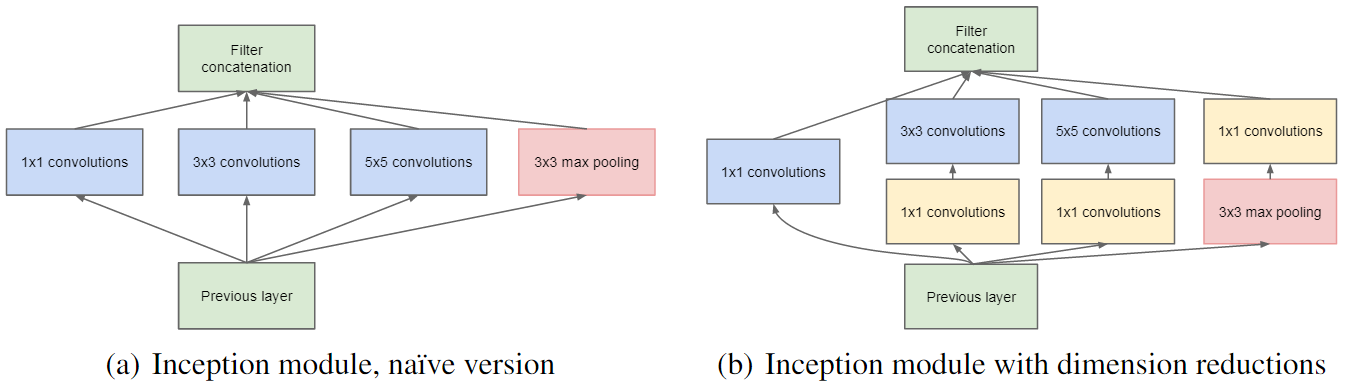
\includegraphics[scale=0.4]{img/inception_1x1.png}
    \end{center}
    \caption{Module Inception \cite{renset}}
    \label{refhinh11}
    \end{figure}
\end{center}
\item Một tích chập 1x1 với 128 bộ lọc để giảm kích thước và tinh chỉnh các đơn vị tuyến tính
\item Một lớp kết nối hoàn chỉnh với 1024 đơn vị và tinh chỉnh các đơn vị tuyến tính.
\item Một tầng loại bỏ (dropout layer) 70\% tỷ lệ đầu ra.
\item Một lớp tuyến tính với tổn thất softmax như là phân loại (dự đoán các lớp 1000 tương tự như phân loại chính, nhưng loại bỏ tại thời gian suy luận  
\end{itemize}

Đây là một trong những kiến trúc CNN đầu tiên thực sự bị lạc khỏi cách tiếp cận tổng quát của việc xếp chồng lên nhau và xếp các lớp lên nhau theo cấu trúc tuần tự. Các tác giả của nhấn mạnh rằng mô hình mới này chú trọng đến việc sử dụng bộ nhớ và điện năng (Lưu ý quan trọng đôi khi chúng ta cũng quên rằng: xếp tất cả các lớp này và thêm một số lượng lớn các bộ lọc có chi phí tính toán và bộ nhớ, cũng như tăng cơ hội overfitting).

\subsection{Mạng ResNet \cite{renset}}

Như ta đã biết độ sâu có tầm quan trọng đặc biệt trong kiến trúc mạng neuron, nhưng các mạng càng sâu thì càng khó đào tạo.

Vấn đề với độ sâu của mạng tăng lên, độ chính xác bị bão hòa và sau đó giảm nhanh chóng. Sự đi xuống không phải do overfitting, và thêm càng  nhiều lớp vào học sâu dẫn đến lỗi đào tạo cao hơn.

Xem xét vấn đề với một mạng nông hơn. Có một giải pháp cho mô hình sâu hơn bằng cách xây dựng các lớp được sao chép từ mô hình nông hơn, và các lớp thêm vào được ánh xạ nhận dạng. Sự tồn tại của giải pháp xây dựng này chỉ ra rằng một mô hình sâu hơn sẽ không tạo ra lỗi đào tạo cao hơn so với mô hình nông hơn. Một lý do khác cho lý do tại sao ResNet lại này có thể hiệu quả là trong suốt quá trình quay ngược trở lại của backpropagation, gradient sẽ dễ dàng chảy qua đồ thị bởi vì chúng ta có các phép toán cộng, phân phối gradient.

Ý tưởng trong mạng này là sau một khối dư bạn có đầu vào của mình là x đi qua chuỗi conv-relu-conv. Điều này sẽ cho ta hàm số F(x). Kết quả sau đó được thêm vào đầu vào ban đầu x. Gọi đó là H(x) = F(x) + x. Trong CNN truyền thống, H(x) bằng F(x), bây giờ ta không chỉ đơn thuần tính toán sự chuyển đổi thằng từ x sang F(x). Về cơ bản, mô đun mini bên dưới hình ảnh thay đổi một chút đầu vào để có một phiên bản mới của CNN. 

\begin{center}
    \begin{figure}[h!]
    \begin{center}
     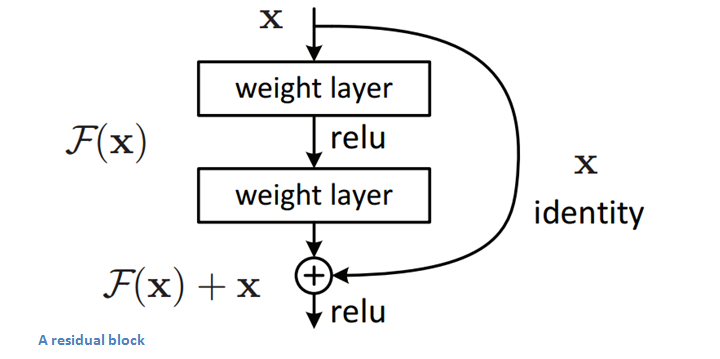
\includegraphics[scale=0.5]{img/ResNet.png}
    \end{center}
    \caption{Một block ResNet \cite{renset}}
    \label{refhinh13}
    \end{figure}
\end{center}

Cho đến năm 2016 thì đây là mạng CNN tốt nhất, giải quyết một phần vấn đề học càng sâu càng tốt.
